\documentclass[12pt, a4paper, oneside, openany]{book}

\usepackage{uomThesisStyle}
\addbibresource{references.bib}

\title{Title of the PDF}
\author{Author Name}
\date{\today}

\makeglossaries{}
\newglossaryentry{G}
{
    name=\(\mathcal{G}\),
    description={Graph},
    sort=G
}
\newglossaryentry{V}
{
    name=\(V\),
    description={The set of nodes},
    sort=V
}
\newglossaryentry{E}
{
    name=\(E\),
    description={The set of links},
    sort=E
}

\newacronym{tcp}{TCP}{Transmission Control Protocol}


\glsaddall{}

\begin{document}

    \frontmatter
    \pagestyle{pageNumbersOnly}

    \begin{titlepage}
    \begin{center}
        \LARGE
        \textbf{Title Goes here}

        Author Name

        
\includegraphics[height=5cm,keepaspectratio]{Figures/umLogo}

        \large
        \textbf{Department of Department Name}

        \textbf{University of Malta}

        \textbf{Month Year}

        \vfill

        \textit{Supervised by}

        \textit{Supervisors Name}

        \vfill

        \textit{Submitted in partial fulfilment of the requirements for the degree of Degree}
    \end{center}
\end{titlepage}
\hypersetup{pageanchor=true}


    \vspace*{\fill}

\begin{center}
    \textbf{Copyright Notice}
\end{center}

\begin{enumerate}
    \item Copyright in text of this thesis rests with the Author.
    Copies (by any process) either in full, or of extracts, may be made only in
    accordance with regulations held by the Library of the University of Malta.
    Details may be obtained from the Librarian.
    This page must form part of any such copies made. Further copies (by any
    process) made in accordance with such instructions may only be made with
    permission (in writing) of the Author.
    \item Ownership of the right over any original intellectual property, which
    may be contained in or derived from this thesis, is vested in the
    University of Malta and may not be made available for use by third parties
    without the written permission of the University, which will prescribe the
    terms and conditions of any such agreement.
\end{enumerate}

\vfill\cleardoublepage{}

    \vspace*{\fill}

\begin{center}
    \textbf{Acknowledgements}
\end{center}

Personal acknowledgements go here.

\begin{center}
    \rule[1mm]{5cm}{1pt}
\end{center}

Research acknowledgements go here.

\vfill\cleardoublepage{}

    \vspace*{\fill}

\begin{center}
    \textbf{Abstract}
\end{center}

The abstract goes here.

\vfill\cleardoublepage{}


    \tableofcontents

    \listoffigures
    \listoftables

    \printglossary[type=\acronymtype,nonumberlist,title=List of Acronyms]
    \printglossary[nonumberlist,title=Glossary of Symbols]

    \mainmatter{}
    \pagestyle{MainMatter}

    \graphicspath{{Chapters/Introduction/Figures/}}

\chapter{Introduction}%
\label{chap:introduction}

The introduction goes here.
The \gls{tcp} is one of the most commonly used internet
protocol~\cite{networksBook}.
Figure~\ref{fig:diamondNetwork} shows a very simple network topology that can be
used to test the \gls{tcp} protocol.
%
\begin{figure}
  \centering
  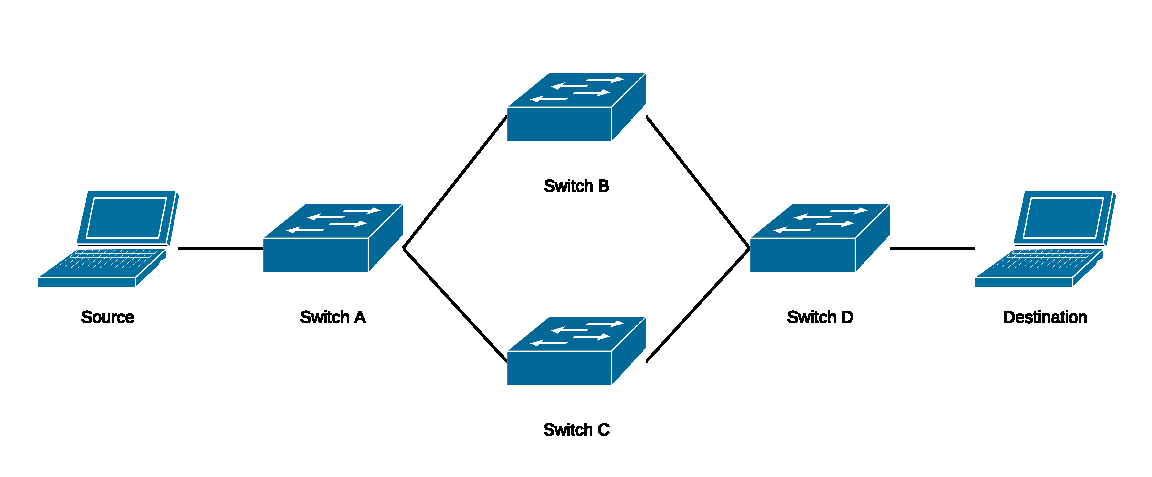
\includegraphics[width=\textwidth,keepaspectratio]{diamondNetwork}
  \caption{Very simple network topology.}%
  \label{fig:diamondNetwork}
\end{figure}
%
Sample results can be found in Table~\ref{tab:sampleTable}.
%
\begin{table}
  \centering
  \caption{Sample Data Table}%
  \label{tab:sampleTable}
  \begin{tabular}{lc}
      \toprule
      Product A & Product B \\
      \midrule
      Item 1    & 100 \\
      Item 2    & 200 \\
      Item 3    & 300 \\
      \bottomrule
  \end{tabular}
\end{table}

    \chapter{Conclusion}%
\label{chap:conclusion}

Conclusion goes here.


    \clearpage

    \pagestyle{pageNumbersOnly}
    \printbibliography[title=References]

    \clearpage

    \pagestyle{MainMatter}
    \appendix
    \chapter{Sample Appendix}%

An appendix goes here.


\end{document}
